\section{Case Study}
\label{case}

The primary motivation for this work is to improve probabilistic forecasts of wind power production, following the framework of \citet{jorgensenSequentialMethodsError2025}. We here use the same same data for a case study. case study,

\subsection{Data}
\label{case-data}

The dataset consists of observed wind-power production and an ensemble of physically based production forecasts for the two Danish electricity bidding zones, DK1 and DK2, each further divided into onshore and offshore wind production.
The two zones differ substantially in geography, installed capacity, and interconnection structure:

\begin{itemize}
    \item DK1 is interconnected with continental Europe.
    \item DK2 is interconnected with the Nordic countries.
\end{itemize}

Each zone exhibits distinct production dynamics, but the time series show clear cross-zone correlation.
Notably, DK1 onshore has by far the largest installed capacity—approximately equal to the other three subzones combined.

A representative example of the full dataset is shown in \cref{caseproduction}.

\begin{figure}[htb]
    \centering
    \includegraphics[width=\linewidth]{Results/Graphs/data_example.pdf}
    \caption{Caption}
    \label{fig:casedata}
\end{figure}

\subsubsection{Observed power Production}
\label{case-data-observed}
Observed production data spans the period
2021‑12‑31 23:00:00 to 2024‑10‑12 22:00:00 (UTC).
Data was obstained from the Danish TSO Energinet, via their open data service
\href{https://www.energidataservice.dk/}{Energi Data Service} \cite{energinetEnergiDataService}.

Energi Data Service provides two similar datasets for energy production, a real-time data set given in 5-minute intervals. and a settlement dataset for statistical  porpuses.

The real-time data set is provided as soon as available, values are based on scaled measurements, thus uncertain, and data errors occur. \cite{energinet_electricityprodex5min_2020}

The statistical dataset is report at hourly intervals and based on settlement data. This dataset is more reliable, but only available at a 9-15 day delay.\cite{energinet_production_consumption_settlement_2020}

For this case study it was chosen to use data set for statistical purposes.

A statistical summary of the observed production for all four zones is provided in \cref{tab:data:observation}.

\begin{table}[htb]
\begin{tabular}{lrrrr}
\toprule
 & DK1-offshore & DK1-onshore & DK2-offshore & DK2-onshore \\
\midrule
mean & 599.49 & 1058.72 & 425.28 & 197.99 \\
std & 408.40 & 876.60 & 330.13 & 173.08 \\
min & 0.01 & 0.83 & 0.01 & 0.01 \\
25% & 209.92 & 317.97 & 105.30 & 48.56 \\
50% & 590.10 & 836.06 & 369.83 & 147.35 \\
75% & 976.31 & 1606.89 & 754.12 & 319.61 \\
max & 1364.77 & 3556.59 & 983.61 & 684.24 \\
\bottomrule
\end{tabular}
\end{table}


\subsubsection{Ensemble forecast}
The other part of the case data is a proprietary ensemble forecast derived from the ECMWF's (European center for midrange weather forecasts) weather forecasts. And consists of:

\begin{itemize}
    \item 1 high‑probability ensemble (HPE)
    \item 50 perturbed ensemble members, generated by perturbing the initial conditions of the HPE.
\end{itemize}

 The ECMWF Forecast is provided at hourly resolution, With the forecast for the day ahead, being made at 12:00 the day before, and several hours after. \cite{ecmwf_about_forecasts}

The individual ensemble members are converted into production forecasts using a proprietary method. Due to the proprietary nature of the method, the ensemble data cannot be disclosed. In iaddition to this case study we also make a simulation study described in \cref{simulation}

\subsubsection{Data anomelies}

Some problematic effects exists in the data.

First is the problem of curtailment. At certain times, producers are paid to reduce generation due to market or transmission constraints, leading to artificially low production values \cite{olson2014a}. In the prior work by \citet{jorgensenSequentialMethodsError2025} These periods of curtailment were remove from the data, as they are not representative of the normal system behaviour.

In addition the ensemble forecast has clear problems in the zone DK2-onshore. In this zone the ensembles occasional collapse to a value $\approx  315 MWh$. These periods where likewise removed in the paper by \citet{jorgensenSequentialMethodsError2025}.

For this case study we keep these periods in. Removing the periods would introduce further problems of missing data, or discontinuous time intervals. 

\subsection{Data Cleaning}

Only light preprocessing of data was necessary:

\begin{itemize}
    \item Zero‑valued observations: Observations equal to exactly zero lead to numerical instability during the probability‑integral-transform stage of the pipeline. To avoid this, values of 0 were replaced with a small positive constant (0.01), which is practically indistinguishable at operational scales.
    \item Timestamp harmonization: the observational and ensemble datasets used slightly different time formats. Both were converted to UTC to ensure alignment
\end{itemize} 

No additional filtering or smoothing was applied.

\subsection{Data Split}

We adopt a straightforward temporal train–test split, ensuring both train- and test set was non-overlapping and uninterrupted intervals. \cite[cp. 3]{theodoridis2020a}

The split was chosen such that there was one year of data in the test set, allowing evaluation across all seasons as wind‑power production exhibits strong seasonal variability\cite{wan2012a}.

The split Was chosen as 53.3\%-46.7\% train-test with the data split at 2023-02-23-22 giving 9983 time points ($\approx$ 416 days) in the train set and 8760 time points ($\approx$ 365 days) in the test set

\subsection{Procedure}
Each zone is modeled independently, meaning:

\begin{itemize}
    \item one marginal quantile model per zone
    \item one correlation (SARIMA) model per zone
    \item no cross‑zone information is used
\end{itemize}

The marginal models use the ensemble forecast at the current time and up to lag 48 hours as covariates:

\[
X_t = [\mathbf{x}_t, x_{t-1},\dots, x_{t-48}]
\]

where  $\mathbf{x}_t \in\mathbb{R}^{51} $ are the 51 individual ensemble members at time t.

Only ensemble information is used as covariates; no observational data enters the forecast at prediction time. This mirrors operational conditions for ensemble‑based forecasting.

To ensure our correlation corrected forecast is made without additional information the stationary distribution of the SARIMA model should be used. due to implementational constraints, we instead forecasted a long "burn-in" period (h = 10000) was simulated, only data points after the burn-in period.

For evaluating scores k = 1000 simulations was made from each model, in normal space. To compare performace scores for the pure marginal models were also calculated. For these models random iid. sample were drawn from a standard normal distribution then converted back into original space.

For comparison the scores for the ensembles were also calculated, This was done using only the 51 ensembles, The result of which is therefore more uncertain.

\subsection{Results}

An example of the forecast provided by the method can be seen in \cref{fig:forecastexample}. Where the correlation corrected forecast is provided. The period visualised is the same as in \cref{fig:casedata} for comparison purpose.

\begin{figure}
    \centering
    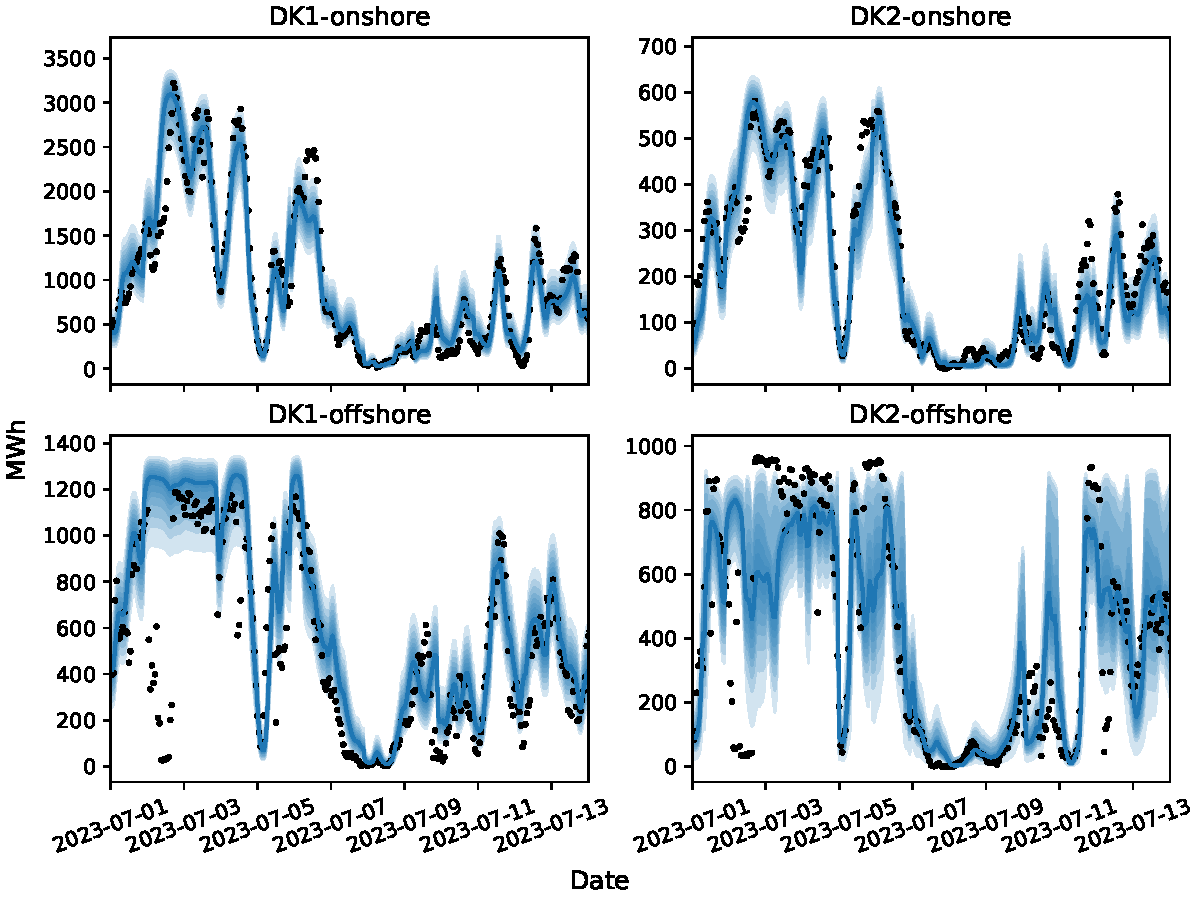
\includegraphics[width=1\linewidth]{Results/Graphs/corrolation_example.pdf}
    \caption{Caption}
    \label{fig:forecastexample}
\end{figure}

The loss curves during the training of the neural nets can be seen in \cref{fig:loss}. Showing both the training and validation loss.

\begin{figure}
    \centering
    \includegraphics[width=1\linewidth]{Results/Graphs/loss_curves.pdf}
    \caption{Caption}
    \label{fig:loss}
\end{figure}

To inform SARIMA model structure. The ACF and PACf for the pseudoresiduals are plotted in \cref{fig:acf_pacf} both before an after applying the correlation models.

\begin{figure}
    \centering
    \includegraphics[width=1\linewidth]{Results/Graphs/acf_pacf.pdf}
    \caption{Caption}
    \label{fig:acf_pacf}
\end{figure}


For the SARIMA models the estimated parameters are found in \cref{tab:parameters}. Where parameters estimated using both the simple- and latent model are presented.

\begin{tabular}{lrrrrrrrr}
\toprule
 & \multicolumn{2}{r}{DK1-onshore} & \multicolumn{2}{r}{DK2-onshore} & \multicolumn{2}{r}{DK1-offshore} & \multicolumn{2}{r}{DK2-offshore} \\
 & Latent & Simple & Latent & Simple & Latent & Simple & Latent & Simple \\
\midrule
ar1 & 0.83 & 0.79 & 0.83 & 0.83 & 0.80 & 0.82 & 0.83 & 0.86 \\
\cline{1-9}
ma1 & 0.30 & 0.01 & 0.24 & 0.19 & 0.20 & 0.11 & 0.26 & 0.33 \\
\cline{1-9}
AR1 & 0.11 & 0.05 & 0.05 & 0.05 & 0.02 & 0.03 & -0.00 & -0.01 \\
\cline{1-9}
sigma & 0.16 & 0.37 & 0.21 & 0.21 & 0.21 & 0.23 & 0.18 & 0.14 \\
\cline{1-9}
\bottomrule
\end{tabular}


The finally performance metrics for all zones and models are presented in \cref{tab:scores}. showing the raw ensemble scores, as well as model scores as a percentage of the ensemble scores.

\begin{tabular}{llrrrrr}
\toprule
 &  & Ensembles & Latent & Latent - Marginal & Simple & Simple - Marginal \\
\midrule
\multirow[c]{5}{*}{DK1-offshore} & MAE & 138.74 & 118.90 & 119.00 & 116.75 & 116.64 \\
\cline{2-7}
 & RMSE & 193.46 & 176.06 & 176.20 & 171.69 & 171.69 \\
\cline{2-7}
 & CRPS & 107.67 & 87.09 & 86.80 & 86.52 & 86.69 \\
\cline{2-7}
 & VarS & 29.65 & 26.36 & 31.90 & 26.50 & 33.44 \\
\cline{2-7}
 & Geometric Mean Score & 96.21 & 83.26 & 87.29 & 82.33 & 87.29 \\
\cline{1-7} \cline{2-7}
\multirow[c]{5}{*}{DK1-onshore} & MAE & 192.07 & 181.74 & 181.89 & 201.67 & 201.67 \\
\cline{2-7}
 & RMSE & 263.32 & 258.65 & 259.08 & 282.17 & 282.17 \\
\cline{2-7}
 & CRPS & 138.56 & 131.14 & 132.11 & 149.22 & 148.53 \\
\cline{2-7}
 & VarS & 36.60 & 36.38 & 49.99 & 52.55 & 66.92 \\
\cline{2-7}
 & Geometric Mean Score & 126.55 & 122.38 & 132.82 & 145.34 & 154.22 \\
\cline{1-7} \cline{2-7}
\multirow[c]{5}{*}{DK2-offshore} & MAE & 158.55 & 124.73 & 124.46 & 141.50 & 141.39 \\
\cline{2-7}
 & RMSE & 239.70 & 181.04 & 181.03 & 206.90 & 206.89 \\
\cline{2-7}
 & CRPS & 124.22 & 88.32 & 88.70 & 99.16 & 99.26 \\
\cline{2-7}
 & VarS & 30.68 & 30.49 & 42.55 & 31.94 & 45.57 \\
\cline{2-7}
 & Geometric Mean Score & 109.71 & 88.31 & 96.03 & 98.13 & 107.25 \\
\cline{1-7} \cline{2-7}
\multirow[c]{5}{*}{DK2-onshore} & MAE & 82.52 & 39.85 & 39.86 & 38.26 & 38.23 \\
\cline{2-7}
 & RMSE & 112.76 & 55.90 & 55.96 & 52.92 & 52.88 \\
\cline{2-7}
 & CRPS & 63.68 & 28.68 & 28.76 & 28.36 & 28.63 \\
\cline{2-7}
 & VarS & 10.30 & 8.27 & 10.75 & 8.33 & 12.07 \\
\cline{2-7}
 & Geometric Mean Score & 49.71 & 26.96 & 28.82 & 26.30 & 28.91 \\
\cline{1-7} \cline{2-7}
\bottomrule
\end{tabular}
